\documentclass[11pt]{article}% uses letterpaper by default

%---------- Uncomment one of them ------------------------------
\usepackage[includeheadfoot, top=0.5in, bottom=0.5in, hmargin=1in]{geometry}

\usepackage{fancyhdr}
\usepackage{setspace}
\renewcommand{\footrulewidth}{0.4pt}% default is 0pt
\usepackage[makeroom]{cancel}
\pagestyle{fancy}
\usepackage{graphicx}
\singlespacing
\usepackage{amsmath}

\newcommand{\SPACE}{\vspace{6em}}
\newcommand{\degrees}{\ensuremath{^\circ}}
\newcommand{\arcmin}{\ensuremath{'}}
\newcommand{\arcsec}{\ensuremath{"}}
\newcommand{\hours}{\ensuremath{^\mathrm{h}}}
\newcommand{\minutes}{\ensuremath{^\mathrm{m}}}
\newcommand{\seconds}{\ensuremath{^\mathrm{s}}}
\newcommand{\labnumber}{05}  % UPDATE THIS!

\usepackage{datetime2}  % customize \today, defaults to yyyy-mm-dd
\lhead{ASTR UN1903 -- Lab \labnumber}
\lfoot{M. Sayeed}
\cfoot{\thepage}
\rfoot{\today}
\rhead{Mondays 6-9 pm}
\renewcommand{\rightmark}{}
\renewcommand{\headrulewidth}{0pt}
\renewcommand{\footrulewidth}{0.4pt}
% -----------------------------
% End personal config (AT, Sp 2019)
% -----------------------------

\usepackage[colorlinks=true,urlcolor=magenta,linkcolor=blue]{hyperref}
% urlcolor = URL links, linkcolor = within-PDF links

\newcommand*{\mt}{\mathrm}
\newcommand*{\unit}[1]{\;\mathrm{#1}}  % vemod.net/typesetting-units-in-latex
\newcommand*{\Msun}{\mathrm{M}_{\sun}}

% Compact spacing
\setlength\parindent{0pt}
\setlength{\parskip}{1em}

% -----------------------------
% End personal config (AT, Sp 2019)
% -----------------------------


\begin{document}

\begin{center}
\Large\textbf{Lab \labnumber: The Earth-Moon-Sun System}
\end{center}

\section{Introduction}

Today you will explore Earth's rotation and its revolution around the Sun. You'll also study the Moon, which is Earth's only natural satellite and the brightest object in the night sky (and therefore a regular nuisance to astronomers).

As a warm-up, briefly discuss the following questions with your neighbors and write
down the answers in your notebook.
\begin{enumerate}
\item How long does it take the Earth to rotate once on its own axis?
\item How long does it take the Earth to revolve once around the Sun?
\item The Sun rises in the East and sets in the West. Which way does the Earth rotate?
\item What causes the seasons?
\item What causes the Moon's phases?
\end{enumerate}


\section{Earth's Rotation}
In this section, you will model the Earth's rotation.  The lamp (or flashlight) is the Sun. Your head, for now, will represent Earth.

Figure out these questions as a group, but no need to write down the answers.
\begin{itemize}
	\item Take a practice rotation to determine your axis of rotation.
	\item Where is the North pole in this model? The South pole?
	\item Where is the equator?
	\item How do you experience 'daytime' and 'nighttime' in this model?
	\item How can you control the length of the day in your model?
\end{itemize}

In your notebooks, explain how the following are represented in your model system:
\begin{enumerate}
	\item Earth's rotation about its own axis
	\item Earth's revolution around the Sun
	\item The North Pole
\end{enumerate}

Pretend there is a microbe-sized person standing on the tip of your nose.
Their feet are flat on your nose, and they face the floor.
Discuss and figure out the following as a group, no need to write in your
notebook.
\begin{itemize}
	\item What is directly over this person's head?
	\item Where is their horizon? (What are the edges of their field of view?)
	\item Where should the Sun rise and set for them? (Which way is East and which way is West?  It may help if you visualize sunrise/sunset the way you would see them from Manhattan facing South.)
	\item How would your answers to the previous questions change if the person were standing on top of your head instead of on your nose?
\end{itemize}

Determine what time it is in your city (i.e., your nose) when you stand in the following positions; record answers in your notebook.
\begin{enumerate}
	\item Facing the Sun
	\item Facing directly away from the Sun
	\item With your right shoulder towards the Sun
    \item Sketch a diagram showing your ``Face-Earth'' and the Sun from above, and indicate clearly on the diagram which direction you would need to be facing in order for it to be the following times in your ``Nose-City'': 6 am, Noon, 3 pm.
\end{enumerate}

\section{The Moon's Phases}
Now we'll return to our personal model from Section 1 and discuss the phases of the Moon. Everyone will get a styrofoam ball with a stick -- this is your Moon, and your head will again be Earth.

In your groups, take turns having someone hold the ``Moon'' and rotate around the ``Earth'' counterclockwise until they complete a full circle.  While doing this, ``Earth'' should rotate while always facing the ``Moon'' to see what the ``Moon'' looks like at any given time from Earth. Note which part of the Moon is bright and which is dark at any given time.  Repeat this until everyone gets a chance to be ``Earth''.

\begin{enumerate}
    \item In the moon-phase diagram (back of lab), draw the shape of the Moon in each position. Clearly mark which is the bright and which is the dark part of the Moon in your drawings.
    \item Can you recognize the phases of the Moon? Which configuration gives a full moon? Which gives a new Moon (when you can only see the dark side of the Moon)? Indicate them in your diagram.
    \item When does the Moon rise and set when it's at positions 1, 3, and 5?
\end{enumerate}
Turn in this diagram with your report.

\section{Earth's Revolution}
Okay, time to use the globes: they will represent...well, guess. We'll use the globes to see how the amount of sunlight hitting different regions of the Earth changes as Earth goes around the sun. Keep the North pole of the globe pointed at the ``North Star'' (the Northern wall/ceiling of the library, with the old desktop computers). The Earth's axis of rotation is slightly tilted (20 degrees) with respect to its orbital plane around the Sun; be sure to account for this effect.

\begin{enumerate}

\item The globe has New York marked on it. First, determine which way you need to spin the globe in order for sunrise and sunset to appear in the right directions. \textbf{Make a diagram showing your setup from above, as well as the direction of Earth's rotation around its own axis.} Make sure to leave enough room in your diagram for the Earth to revolve all the way around the Sun!
%Also, indicate in your diagram which way your model is set
%up with respect to the classroom.

\item Find the points in Earth's orbit around the Sun where the Northern Hemisphere points toward and away from the Sun. Label those points clearly in your diagram, adding a small sketch that illustrates how the Earth is tilted with respect to the Sun in each location.

\item Find Santiago, Chile on the globe.  Use these two cities to compare the relative times of sunrise/sunset and the relative lengths of the days, when the Earth's Northern Hemisphere points \textbf{toward} and \textbf{away} from the Sun.

\item Move the globe around the Sun until you find the points in Earth's orbit where the following four events happen in New York City. Note that the Earth orbits the Sun counterclockwise as viewed from the Northern hemisphere.
    \begin{itemize}
    \item Winter Solstice (shortest day of the year)
    \item Summer Solstice (longest day of the year)
    \item Vernal (Spring) Equinox (day and night are equal length)
    \item Autumnal (Fall) Equinox (day and night are equal length)
    \end{itemize}
\item In your notebook, sketch the Sun and show Earth's position at each of the four locations above (you should have already added two of these positions to your diagram in one of the previous questions -- if so, just add the other two). Add a small sketch that illustrates how the Earth is tilted with respect to the Sun in each location, and be sure to label Earth's axis of rotation and both hemispheres.

\item On the equinoxes, which city -- New York or Santiago -- experiences a longer day?

\item What causes the seasons on Earth?

\item Over a full year, does one of the cities receive more sunlight than another?

\item Does noon occur at the same time in both cities?  In which season does each city experience more direct sunlight (more direct sunlight = shorter shadows)?

\item Why is the average temperature at the equator higher than it is at the North Pole?

\end{enumerate}

\newpage
\pagebreak

% \section{Observing the Moon}

% \subsection{Using the Telescope}

% The observing TA will help you use the telescope in the Big Dome.

% %Mathew will explain to you how to use the Dobsonians (``dobs''). Once you're set free, do the following:
% \begin{itemize}

%     \item Use the arrow keys to practice moving the telescope.
%         %Watch how up, down, left, right alter the telescope's position.

%     \item Point to the moon, as a group, using the finder mounted on the side of the telescope.

%     \item Everyone should look through the eyepiece of the telescope and practice adjusting both telescope pointing and focus. The observing TA will help you out.

%     \item The observing TA will place a DSLR camera on the telescope. Take a picture!
%         %We'll distribute electronic and/or printed copies for you to use in the
%         %last part of the lab.
%     Note: this part may be skipped if the eyepiece/camera setup is troublesome to swap around, in which case we'll provide a pre-taken image.

%     \item In your notebook, answer the following:
%         \begin{enumerate}
%             \item The view in the eyepiece differs from your naked eye view.
%                 Besides magnification, what's the difference?
%             \item As you observe, you'll have to keep moving the telescope.
%                 What's going on?  Explain.
%         \end{enumerate}
% \end{itemize}

% \subsection{A picture of the Moon}

% \begin{enumerate}
%     %\item Using the map below, label as many features of the surface of the
%     %    moon as you can in your image.

%     \item What phase is the moon in?  Why does that make it a good night for us to observe? (think about the connection between moon phase and the time it rises and sets)

%     \item On which part of the moon are shadows the longest?  Why is this?

%     \item What parts of the moon do you think are older or younger, and why?

% \end{enumerate}
\section{Seasons}
\begin{enumerate}
    \item Someone tells you that summer occurs when Earth is closer to the sun; winter occurs when Earth is farther. What's wrong with their explanation? Explain how the seasons work, as if you were trying to convince this person in real life.

    \item A lunar eclipse happens when the Earth blocks the Sun from shining on the moon. A solar eclipse happens when the Moon blocks the Sun from shining on the Earth. Draw the Earth-Moon-Sun configuration for each case. What is the phase of the Moon at solar eclipse? Lunar eclipse? Why don't eclipses happen monthly?

\end{enumerate}
\section{Conclusions}
\begin{itemize}
\item What did you like or dislike about this lab?  
\item Any feedback/suggestions?
\item Any remaining questions?
\end{itemize}

\begin{center}
\begin{figure}
    \centering
    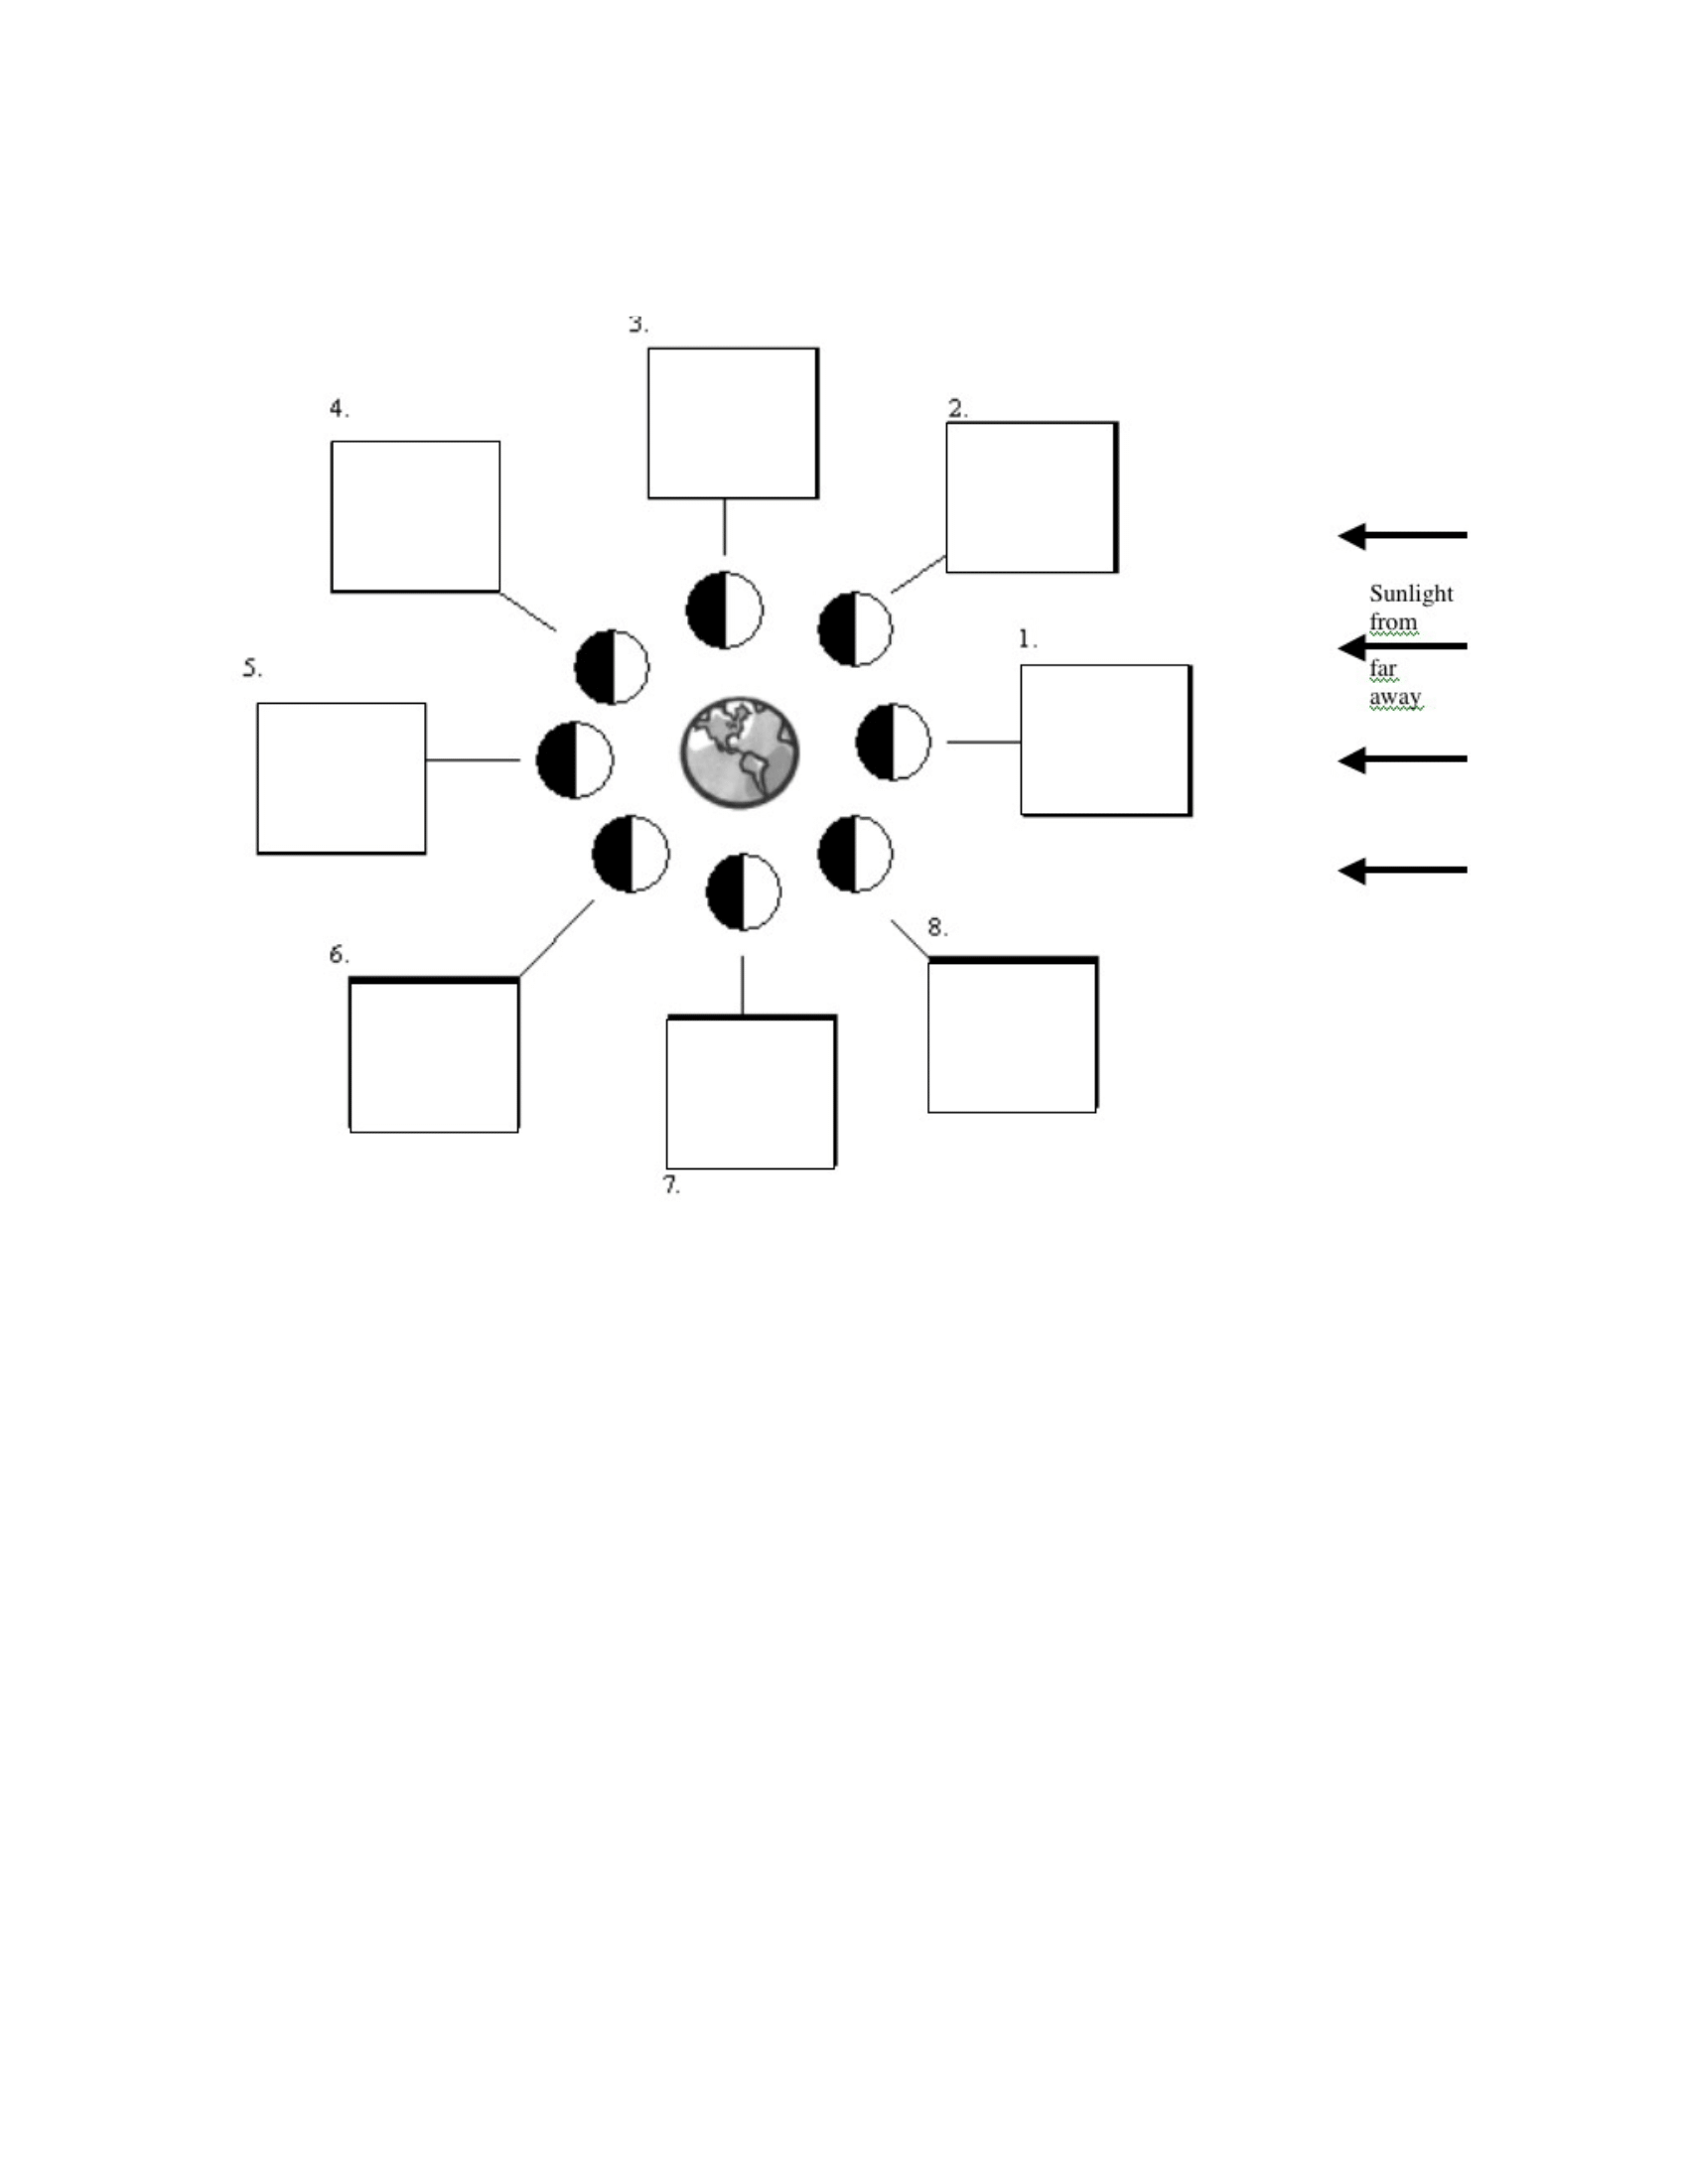
\includegraphics[width=1.1\textwidth]{moon_diagram.png}
    \label{fig:my_label}
\end{figure}
    
\end{center}
\end{document}